%!TEX program = xelatex

\documentclass[compress]{beamer}
%--------------------------------------------------------------------------
% Common packages
%--------------------------------------------------------------------------

\definecolor{links}{HTML}{663000}
\hypersetup{colorlinks,linkcolor=,urlcolor=links}

\usepackage[english]{babel}
\usepackage{pgfpages} % required for notes on second screen
\usepackage{graphicx}

\usepackage{pdfpcnotes}

\usepackage{multicol}

\usepackage{tabularx,ragged2e}
\usepackage{booktabs}

\setlength{\emergencystretch}{3em}  % prevent overfull lines
\providecommand{\tightlist}{%
  \setlength{\itemsep}{0pt}\setlength{\parskip}{0pt}}


\usetheme{hri}

% Display the navigation bullet even without subsections
\usepackage{remreset}% tiny package containing just the \@removefromreset command
\makeatletter
\@removefromreset{subsection}{section}
\makeatother
\setcounter{subsection}{1}

\makeatletter
\let\beamer@writeslidentry@miniframeson=\beamer@writeslidentry
\def\beamer@writeslidentry@miniframesoff{%
  \expandafter\beamer@ifempty\expandafter{\beamer@framestartpage}{}% does not happen normally
  {%else
    % removed \addtocontents commands
    \clearpage\beamer@notesactions%
  }
}
\newcommand*{\miniframeson}{\let\beamer@writeslidentry=\beamer@writeslidentry@miniframeson}
\newcommand*{\miniframesoff}{\let\beamer@writeslidentry=\beamer@writeslidentry@miniframesoff}
\makeatother



\newcommand{\source}[2]{{\tiny\it Source: \href{#1}{#2}}}

\usepackage{tikz}
\usetikzlibrary{mindmap,backgrounds,positioning,calc,patterns}
\usepackage{pgfplots}
\pgfplotsset{compat=newest}
\usepackage{circuitikz}

\graphicspath{{figs/}}

\title{ROCO222 \newline Intro to Sensors and Actuators}
\subtitle{Magnets, Brushless Motors, Motor control}

\date{}
\author{Séverin Lemaignan}
\institute{Centre for Neural Systems and Robotics\\{\bf Plymouth University}}

\begin{document}

\licenseframe{github.com/severin-lemaignan/module-mobile-and-humanoid-robots}

\maketitle

\miniframesoff

\begin{frame}[fragile]{Last week's programming challenge}

    \Large
    Console-based image viewer

        \begin{center}
            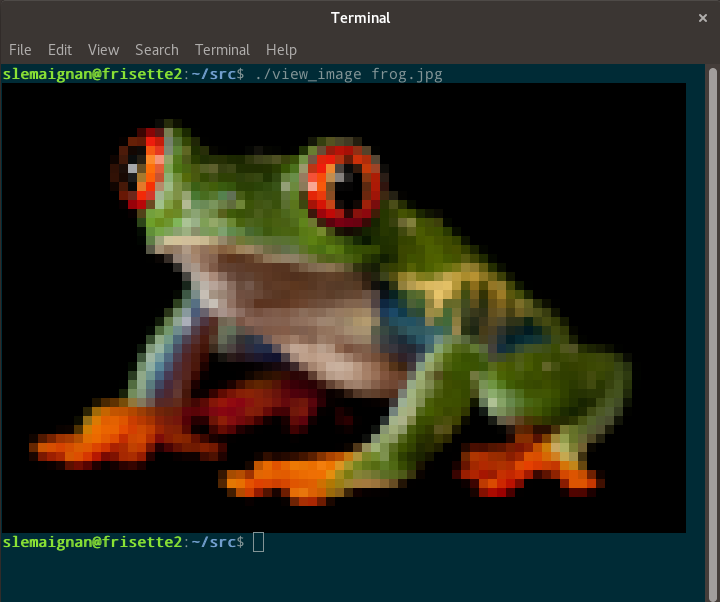
\includegraphics[width=0.7\linewidth]{../part3/figs/coding-challenge-terminal-image}
        \end{center}

\end{frame}

\begin{frame}{Today's objectives}

    \begin{itemize}
        \item Know a bit more about permanent magnets, and in particular, about
            hysteresis curves
        \item Undertand the working principle of a \textbf{brushless motor} and
            how it compares to brushed DC motors
        \item Know what PWM and H-bridge stand for, how a H-bridge is built, and
            how to control it,
        \item Understand the difference between open-loop and closed-loop
            control.

    \end{itemize}
\end{frame}

\miniframeson

%%%%%%%%%%%%%%%%%%%%%%%%%%%%%%%%%%%%%%%%%%%%%%%%%%%%%%%%%%%%%%%%%%
%%%%%%%%%%%%%%%%%%%%%%%%%%%%%%%%%%%%%%%%%%%%%%%%%%%%%%%%%%%%%%%%%%
%%%%%%%%%%%%%%%%%%%%%%%%%%%%%%%%%%%%%%%%%%%%%%%%%%%%%%%%%%%%%%%%%%

\section[Magnets]{Magnetism \& magnets}

{\fullbackground[scale=0.9,page=49]{ian-electromagnetism.pdf}
\begin{frame}{Types of magnetism: paramagnetism}

\end{frame}
}

{\fullbackground[scale=0.9,page=50]{ian-electromagnetism.pdf}
\begin{frame}{Types of magnetism: paramagnetism}

\end{frame}
}
{\fullbackground[scale=0.9,page=51]{ian-electromagnetism.pdf}
\begin{frame}{Types of magnetism: diamagnetism}

\end{frame}
}
{\fullbackground[scale=0.9,page=52]{ian-electromagnetism.pdf}
\begin{frame}{Types of magnetism: ferromagnetism}

\end{frame}
}
{\fullbackground[scale=0.9,page=53]{ian-electromagnetism.pdf}
\begin{frame}{Types of magnetism: ferromagnetism}

\end{frame}
}
{\fullbackground[scale=0.9,page=55]{ian-electromagnetism.pdf}
\begin{frame}{Permanent sources of magnetism}

\end{frame}
}
{\fullbackground[scale=0.9,page=56]{ian-electromagnetism.pdf}
\begin{frame}{Earth's magnetic field}

\end{frame}
}
{\fullbackground[scale=0.9,page=57]{ian-electromagnetism.pdf}
\begin{frame}{Ferrite magnets}

\end{frame}
}
{\fullbackground[scale=0.9,page=58]{ian-electromagnetism.pdf}
\begin{frame}{Alinico (AlNiCo)}

\end{frame}
}
{\fullbackground[scale=0.9,page=59]{ian-electromagnetism.pdf}
\begin{frame}{Samarium cobalt (SmCo)}

\end{frame}
}
{\fullbackground[scale=0.9,page=60]{ian-electromagnetism.pdf}
\begin{frame}{Neodymium magnets (NdFeB)}

\end{frame}
}
{\fullbackground[scale=0.9,page=61]{ian-electromagnetism.pdf}
\begin{frame}{Neodymium magnets are very powerful}

\end{frame}
}
{\fullbackground[scale=0.9,page=62]{ian-electromagnetism.pdf}
\begin{frame}{Magnetization or B-H curve of ferromagnetic materials}

\end{frame}
}
{\fullbackground[scale=0.9,page=63]{ian-electromagnetism.pdf}
\begin{frame}{Magnetic hysteresis loop}

\end{frame}
}
{\fullbackground[scale=0.9,page=64]{ian-electromagnetism.pdf}
\begin{frame}{Important characteristic of permanent magnets}

\end{frame}
}
{\fullbackground[scale=0.9,page=65]{ian-electromagnetism.pdf}
\begin{frame}{Hard and soft magnetic materials}

\end{frame}
}

\begin{frame}{Magnetic hysteresis loops for soft and hard materials}
    \begin{center}
        \includegraphics<1>[width=0.8\linewidth]{hysteresis-soft}
        \includegraphics<2>[width=0.8\linewidth]{hysteresis-soft-hard}
    \end{center}
\end{frame}

{\fullbackground[scale=0.9,page=68]{ian-electromagnetism.pdf}
\begin{frame}{Making a permanent magnet}

\end{frame}
}

{\fullbackground[scale=0.9,page=69]{ian-electromagnetism.pdf}
\begin{frame}{Demagnetizers}

\end{frame}
}

%%%%%%%%%%%%%%%%%%%%%%%%%%%%%%%%%%%%%%%%%%%%%%%%%%%%%%%%%%%%%%%%%%
%%%%%%%%%%%%%%%%%%%%%%%%%%%%%%%%%%%%%%%%%%%%%%%%%%%%%%%%%%%%%%%%%%
%%%%%%%%%%%%%%%%%%%%%%%%%%%%%%%%%%%%%%%%%%%%%%%%%%%%%%%%%%%%%%%%%%
\section[Brushless motors]{Brushless DC motors}

{\fullbackground[scale=0.9,page=2]{../part3/figs/ian-brushless-dc-motors.pdf}
\begin{frame}{Problems of mechanical commutation}

%Can get potential difference across commutator segments
%
%\begin{itemize}
%
%\item Can get potential difference across commutator segments
%\item Commutation shorts out the commutator segments
%\item Arcing and sparkling at the brushes
%\item Brushless electronic switching solves this issue
%\end{itemize}

\end{frame}
}

\begin{frame}{Brushless DC Motor}

    \begin{columns}
        \begin{column}{0.7\linewidth}
\begin{itemize}
\small
\item looks like DC brushed motor turned inside out
\item commutation is performed electronically  to
  eliminate brushes $\rightarrow$ \textbf{electronic commutation, EC}
\item the stator generally consists of several coils
\item current flow in the stator coils creates magnetic field
\item this forces the permanent magnet rotor to spin
\item continuous rotation by switching on current
    in the stator $\rightarrow$ \textbf{sequenced magnetic field}
\item brushless motors \textbf{require a controller} that perform the commutation
\end{itemize}
            
        \end{column}
        \begin{column}{0.3\linewidth}
            \begin{center}
                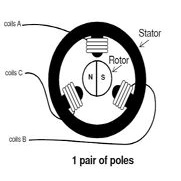
\includegraphics[width=\linewidth]{../part3/figs/brushless-schematic}
            \end{center}
        \end{column}
    \end{columns}

\end{frame}

\imageframe[caption=Typical brushless motor,scale=0.9]{../part3/figs/image81}


{\fullbackground[scale=0.9,page=5]{../part3/figs/ian-brushless-dc-motors.pdf}
\begin{frame}{How do brushless motors work?}

%\begin{itemize}
%\item Electronic commutation is used to switch current in the stator could
%  so that the rotor is forced to rotate
%\item There is often a control magnet is in line with the poles of the large
%  magnet in the motor to identify rotor angle so that the controller can
%  switch current into the appropriate coils
%\item As it turns Hall sensors are stimulated by the magnetic flux.
%\item The Hall sensors are used to tell the controller what the orientation
%  is of the magnet with respect to the three winding phases.
%\item Current in the stator coils is turned on and off in sequence creating
%  motion from pole to pole.
%\end{itemize}

\end{frame}
}

\videoframe[0.65]{../part3/figs/brushless-commutation.mp4}

%{\fullbackground[scale=0.9,page=21]{../part1/figs/ian-sensors.pdf}
%    \begin{frame}{Electronic commutation systems}
%    \note {
%In this third part of the presentation we would like to understand the electronic commutation.
%There are different systems. maxon uses the following three :
%
%- Block commutation with or without Hall sensors
%- Sinusoidal commutation.
%
%As you can see the different maxon controller families perform different commutation types.
%
%Common to all these systems is that they should apply the current in a way, that the generated torque is as high as possible. As we have learned this is achieved by a perpendicular orientation of the magnetic fields of permanent magnet and winding. We have seen as well that we need to know the orientation of the permanent magnet to achieve this.
%
%We start with block commutation with Hall sensor position feedback. That's the standard commutation type. Once we have understood this the two other commutation schemes are easily derived from it.
%    }
%    \end{frame}
%}

{\fullbackground[scale=0.9,page=22]{../part1/figs/ian-sensors.pdf}
    \begin{frame}{Block commutation}

\pnote{
First we have to look at the Hall sensor feedback signals. Again we do this
based on the simplest design, the slotless maxon EC motor with 1 pole pair.

In the back of the motor there are three Hall sensor mounted on the PCB at an
angle of 120°. The Hall sensor detect the magnetic poles of the control magnet
which is mounted on the shaft. The control magnet exhibits the same two
magnetic poles in the same orientation as the power magnet. (Basically the Hall
sensors could monitor the power magnet directly but the control magnet offers
two advantages: The magnetic transitions between north and south pole are more
precisely defined. And an angular misalignment and tolerances between the
relative position of winding and Hall sensors can be adjusted.)

The digital Hall sensors used probe the direction of the magnetic field. They
generates a high output signal (5V) if the north pole of the control magnet is
close to them. A south pole produces a low level (Gnd).

The actual position of the control magnet in the diagram generates the
following signals:

- The blue Hall sensor sees the north pole. Thus the signal output level is
high and will remain high for the next 120°.
- The green Hall sensor is close to the south pole. The output level is low for
the next 60°. Then the north pole approaches and the output signal will switch
to a high state.
- The red Hall sensor has just switched from high to low where the signal level
will stay for the next half a turn.

The combination of the three Hall sensor signals is unique for each 60° of
rotation. Looking at these signals allows to know the rotor position within
60°. That exactly what we need for commutation. Remember there were 6 different
ways of current flow through the motor at a commutation angle of 60°.

The next slide shows how the complete block commutation system works.
}
    \end{frame}
}

{\fullbackground[scale=0.9,page=23]{../part1/figs/ian-sensors.pdf}
    \begin{frame}{Components of an EC drive system}
\pnote{
Let's first look at an EC drive system in general.

The three phases of the EC motor cannot be connected directly to a DC power
supply. The voltage needs to be switched in a sequence. This is done by the
electronic commutation. For the correct switching the electronics needs rotor
position information from the motor. This information is usually provided by
the Hall sensors.

An EC motor cannot operate on its own: It's always the combination of motor and
electronics commutation that makes the full drive.


For more sophisticated commutation and precise motor control, e.g. at very low
speeds, the use of an encoder feedback might be necessary. Often the
electronics not only performs the commutation but at the same time can be used
to control speed or position.
}
    \end{frame}
}



{\fullbackground[scale=0.9,page=7]{../part3/figs/ian-brushless-dc-motors.pdf}
\begin{frame}{Brushless motor for RC aircraft}

\end{frame}
}

{\fullbackground[scale=0.9,page=8]{../part3/figs/ian-brushless-dc-motors.pdf}
\begin{frame}{Construction of a EC brushless motor}

%Permanent magnet
%
%Special Winding
%
%Rotating part -- permanent magnet
%
%Hall sensors
%
%Control Magnet
%
%Case / Magnetic
%
%return

\end{frame}

}

{\fullbackground[scale=0.9,page=9]{../part3/figs/ian-brushless-dc-motors.pdf}
\begin{frame}{Maxon EC flat brushless motor}

%Multi pole motor
%
%Flat design gives more torque as the flux is acting further from the
%centre of rotation

\end{frame}

}

{\fullbackground[scale=0.9,page=10]{../part3/figs/ian-brushless-dc-motors.pdf}
\begin{frame}{Advantages and disadvantages of EC}

%\textbf{Brushed DC motors}
%
%\begin{itemize}
%
%\item Mechanical commutation
%\item Need periodic brush maintenance
%\item Power losses in brushes
%\item Sparking
%\item Can have noisy operation
%\item Linear torque characteristic at lower
%\item Change direction by changing voltage polarity
%\item Controller not always needed
%\end{itemize}
%
%\textbf{EC motors}
%
%\begin{itemize}
%
%\item Electronic commutation
%\item Low or no maintenance
%\item Less power loss
%\item No sparking
%\item Quieter operation
%\item More linear torque characteristic
%\item Change direction by changing switching sequence
%\item Always needs drive controller circuitry
%\item Requires sensors
%\item Higher reliability \& efficiency
%\item Stator on outside -- better for heat dissipation
%\item Longer life
%\item More expensive
%\end{itemize}

\end{frame}
}

%%%%%%%%%%%%%%%%%%%%%%%%%%%%%%%%%%%%%%%%%%%%%%%%%%%%%%%%%%%%%%%%%%
%%%%%%%%%%%%%%%%%%%%%%%%%%%%%%%%%%%%%%%%%%%%%%%%%%%%%%%%%%%%%%%%%%
%%%%%%%%%%%%%%%%%%%%%%%%%%%%%%%%%%%%%%%%%%%%%%%%%%%%%%%%%%%%%%%%%%

\section{Motor control}

{\fullbackground[scale=0.9,page=07]{ian-motor-ctrl.pdf}
    \begin{frame}{Open loop control systems}
    \end{frame}
}

{\fullbackground[scale=0.9,page=08]{ian-motor-ctrl.pdf}
    \begin{frame}{Open loop control systems}
    \end{frame}
}

{\fullbackground[scale=0.9,page=09]{ian-motor-ctrl.pdf}
    \begin{frame}{Simple feedback controller}
    \end{frame}
}

{\fullbackground[scale=0.9,page=10]{ian-motor-ctrl.pdf}
    \begin{frame}{Simple feedback controller}
    \end{frame}
}


\begin{frame}{Four quadrant operation of DC motor}

    In a DC motor, what do we control? 
    
    The speed? The torque?

\end{frame}

\begin{frame}{Four quadrant operation -- hoist example}

    \resizebox{\linewidth}{!}{
    \begin{tikzpicture}[>=latex]
        \node at (0,0) {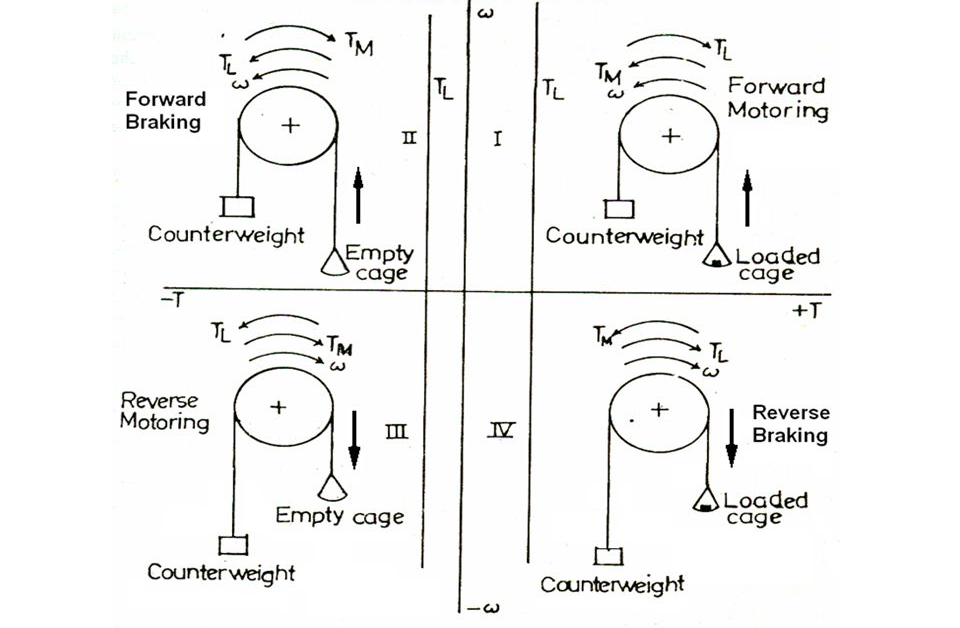
\includegraphics[width=0.9\linewidth]{four-quadrant-hoist}};
        \node at (-6,2) [align=right]{Forward movement, \\motor torque opposite
                                    \\from direction of rotation};
        \node at (6,2) [align=left]{Forward movement, \\motor torque in\\
        direction of rotation};
        \node at (-6,-2) [align=right]{Backward movement, \\motor torque
        in\\direction of rotation};
        \node at (6,-2) [align=left]{Backward movement,\\motor torque opposite
        \\from direction of rotation};
    \end{tikzpicture}
    }


\end{frame}


\begin{frame}{Motor speed-torque chart}

    \begin{columns}
        \begin{column}{0.4\linewidth}
    \begin{center}
        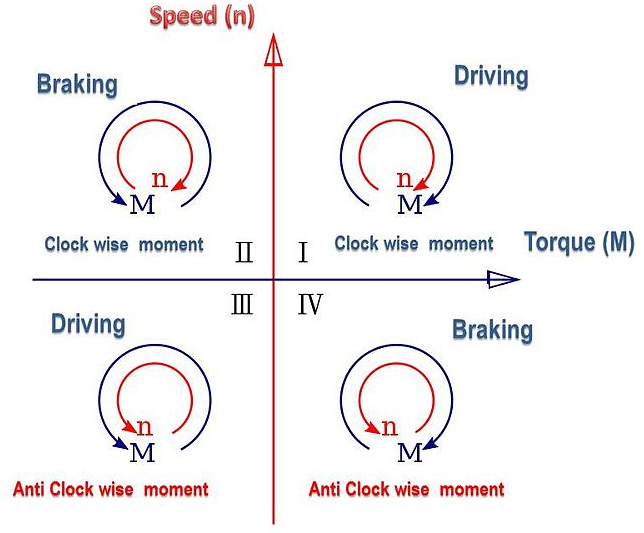
\includegraphics[width=1.1\columnwidth]{four-quadrant}
    \end{center}
            
        \end{column}
        \begin{column}{0.6\linewidth}
    \begin{itemize}
        \item \textbf{Quadrant I} -– Driving forward with positive speed and positive torque
        \item \textbf{Quadrant II} -- Generating or braking with positive speed and negative torque
        \item \textbf{Quadrant III} -– Driving with negative speed and negative torque
        \item \textbf{Quadrant IV} -- Generating or braking with negative speed
            and positive torque. \textbf{Regenerative braking} or
            \textbf{Reverse braking}.

    \end{itemize}

        \end{column}
    \end{columns}


    \source{http://www.electronicshub.org/four-quadrant-operations-of-dc-motor/}{ElectronicsHub
    (check the link for more details)}
\end{frame}

{\fullbackground[scale=0.9,page=03]{ian-motor-ctrl.pdf}
    \begin{frame}{One and two quadrant operation}
    \end{frame}
}

{\fullbackground[scale=0.9,page=05]{ian-motor-ctrl.pdf}
    \begin{frame}{Four quadrant operation}
    \end{frame}
}

\begin{frame}{Relation to the Speed-torque characteristic}

    \begin{columns}
        \begin{column}{0.7\linewidth}
    \begin{center}
        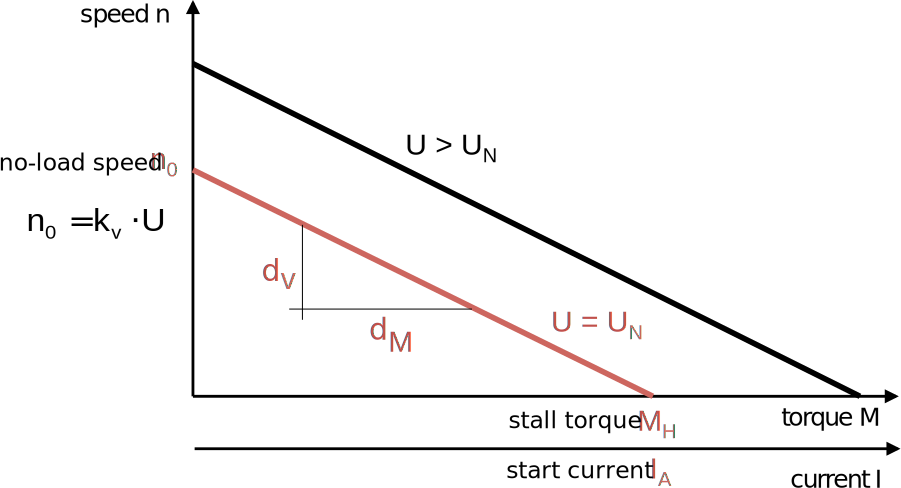
\includegraphics[width=\linewidth]{../part3/figs/voltage-torque}
    \end{center}


        \end{column}
        \begin{column}{0.3\linewidth}
            Remember:

    \begin{align*}
        \dot\theta &= \frac{V}{K} - R \cdot \frac{\tau}{K^2} \\
        \tau &= K \cdot I
    \end{align*}

        \end{column}
    \end{columns}


\end{frame}


\miniframesoff
\begin{frame}[plain]
    \begin{center}
        \Large
        10 min break\\[2em]
    \end{center}
\end{frame}
\miniframeson


%%%%%%%%%%%%%%%%%%%%%%%%%%%%%%%%%%%%%%%%%%%%%%%%%%%%%%%%%%%%%%%%%%
%%%%%%%%%%%%%%%%%%%%%%%%%%%%%%%%%%%%%%%%%%%%%%%%%%%%%%%%%%%%%%%%%%
%%%%%%%%%%%%%%%%%%%%%%%%%%%%%%%%%%%%%%%%%%%%%%%%%%%%%%%%%%%%%%%%%%
\section[Open-loop control]{Open-loop motor control}

{\fullbackground[scale=0.9,page=2]{ian-simple-motor-ctrl.pdf}
    \begin{frame}{Open loop control}
    \end{frame}
}
{\fullbackground[scale=0.9,page=3]{ian-simple-motor-ctrl.pdf}
    \begin{frame}{Closed loop control}
    \end{frame}
}

{\fullbackground[scale=0.9,page=4]{ian-simple-motor-ctrl.pdf}
    \begin{frame}{Motor operating point voltage dependent}
    \end{frame}
}

{\fullbackground[scale=0.9,page=5]{ian-simple-motor-ctrl.pdf}
    \begin{frame}{Simple motor speed control}
    \end{frame}
}

{\fullbackground[scale=0.9,page=6]{ian-simple-motor-ctrl.pdf}
    \begin{frame}{Linear power stage}
    \end{frame}
}

{\fullbackground[scale=0.9,page=7]{ian-simple-motor-ctrl.pdf}
    \begin{frame}{Better motor speed control}
    \end{frame}
}

{\fullbackground[scale=0.9,page=8]{ian-simple-motor-ctrl.pdf}
    \begin{frame}{Pulsed power stage (PWM)}
    \end{frame}
}

{\fullbackground[scale=0.9,page=9]{ian-simple-motor-ctrl.pdf}
    \begin{frame}{Pulse width modulation waveforms}
    \end{frame}
}

{\fullbackground[scale=0.9,page=10]{ian-simple-motor-ctrl.pdf}
    \begin{frame}{PWM and current ripple}
    \end{frame}
}

{\fullbackground[scale=0.9,page=11]{ian-simple-motor-ctrl.pdf}
    \begin{frame}{PWM and electronic commutation}
    \end{frame}
}

\section{H-bridge}

{\fullbackground[scale=0.9,page=02]{ian-hbridge.pdf}
    \begin{frame}{H-bridge}
    \end{frame}
}


{\fullbackground[scale=0.9,page=03]{ian-hbridge.pdf}
    \begin{frame}{H-bridge control motor direction}
    \end{frame}
}


{\fullbackground[scale=0.9,page=04]{ian-hbridge.pdf}
    \begin{frame}{Using junction transistors as switches}
    \end{frame}
}


{\fullbackground[scale=0.9,page=05]{ian-hbridge.pdf}
    \begin{frame}{Motor inductance}
    \end{frame}
}


{\fullbackground[scale=0.9,page=06]{ian-hbridge.pdf}
    \begin{frame}{Back EMF chen current abruptly switched off}
    \end{frame}
}


{\fullbackground[scale=0.9,page=07]{ian-hbridge.pdf}
    \begin{frame}{Diode protection against back EMF}
    \end{frame}
}


{\fullbackground[scale=0.9,page=08]{ian-hbridge.pdf}
    \begin{frame}{Simple transistor H-Bridge}
    \end{frame}
}


{\fullbackground[scale=0.9,page=09]{ian-hbridge.pdf}
    \begin{frame}{H-Bridges are available off-the-shelf}
    \end{frame}
}


\section{Motor control with Arduino}

{\fullbackground[scale=0.9,page=02]{ian-arduino-dc-motors.pdf}
    \begin{frame}{Arduino motor shield}
    \end{frame}
}

{\fullbackground[scale=0.9,page=03]{ian-arduino-dc-motors.pdf}
    \begin{frame}{Arduino motor shield specs}
    \end{frame}
}

{\fullbackground[scale=0.9,page=04]{ian-arduino-dc-motors.pdf}
    \begin{frame}{L298 dual full-bridge driver}
    \end{frame}
}

{\fullbackground[scale=0.9,page=05]{ian-arduino-dc-motors.pdf}
    \begin{frame}{L298 dual full-bridge driver}
    \end{frame}
}

{\fullbackground[scale=0.9,page=06]{ian-arduino-dc-motors.pdf}
    \begin{frame}{Motor shield schematic}
    \end{frame}
}

{\fullbackground[scale=0.9,page=07]{ian-arduino-dc-motors.pdf}
    \begin{frame}{Install the Arduino motor shield}
    \end{frame}
}

{\fullbackground[scale=0.9,page=08]{ian-arduino-dc-motors.pdf}
    \begin{frame}{Arduino motor shield power supply}
    \end{frame}
}

{\fullbackground[scale=0.9,page=09]{ian-arduino-dc-motors.pdf}
    \begin{frame}{Arduino motor shield output channels}
    \end{frame}
}

{\fullbackground[scale=0.9,page=10]{ian-arduino-dc-motors.pdf}
    \begin{frame}{Pins always in use by the motor shield}
    \end{frame}
}

{\fullbackground[scale=0.9,page=11]{ian-arduino-dc-motors.pdf}
    \begin{frame}{Motor shield pin usage}
    \end{frame}
}

{\fullbackground[scale=0.9,page=13]{ian-arduino-dc-motors.pdf}
    \begin{frame}{DC motor connections}
    \end{frame}
}

{\fullbackground[scale=0.9,page=14]{ian-arduino-dc-motors.pdf}
    \begin{frame}{Motor shield 1-channel DC motor demo}
    \end{frame}
}

\begin{frame}[fragile]{Motor shield 1-channel DC motor demo}

\begin{cppcode}
/*****************************************************
Motor Shield 1-Channel DC Motor Demo
by Randy Sarafan
For more information see:
www.instructables.com/id/Arduino-Motor-Shield-Tutorial
*****************************************************/
void setup() {
//Setup Channel A
pinMode(12, OUTPUT); //Initiates Motor Channel A pin
pinMode(9, OUTPUT); //Initiates Brake Channel A pin
}
\end{cppcode}

\end{frame}

\begin{frame}[fragile]{Motor shield 1-channel DC motor demo}

\begin{cppcode}
void loop(){
  //forward @ full speed
  digitalWrite(12, HIGH); //Establishes forward direction of Channel A
  digitalWrite(9, LOW); //Disengage the Brake for Channel A
  analogWrite(3, 255); //Spins the motor on Channel A at full speed
  delay(3000);
  digitalWrite(9, HIGH); //Engage the Brake for Channel A
  delay(1000);
  //backward @ half speed
  digitalWrite(12, LOW); //Establishes backward direction of Channel A
  digitalWrite(9, LOW); //Disengage the Brake for Channel A
  analogWrite(3, 123); //Spins the motor on Channel A at half speed
  delay(3000);
  digitalWrite(9, HIGH); //Engage the Brake for Channel A
  delay(1000);
}
\end{cppcode}

\end{frame}


{\fullbackground[scale=0.9,page=17]{ian-arduino-dc-motors.pdf}
    \begin{frame}{DC motor running}
    \end{frame}
}

{\fullbackground[scale=0.9,page=18]{ian-arduino-dc-motors.pdf}
    \begin{frame}{Motor shield 2-channels DC motor demo}
    \end{frame}
}

\begin{frame}[fragile]{Motor shield 2-channels DC motor demo}

\begin{cppcode}
/*************************************************************
Motor Shield 2‐Channel DC Motor Demo
by Randy Sarafan
  
For more information see:
www.instructables.com/id/Arduino-Motor‐Shield‐Tutorial
*************************************************************/
  
  
void  setup()
{
  //Setup Channel A
  pinMode(12, OUTPUT);  //Initiates  Motor  Channel  A  pin
  pinMode(9,  OUTPUT);  //Initiates  Brake  Channel  A  pin
  
  //Setup  Channel  B
  pinMode(13,  OUTPUT);  //Initiates  Motor  Channel  A  pin
  pinMode(8,  OUTPUT);    //Initiates  Brake  Channel  A  pin
}
\end{cppcode}

\end{frame}

\begin{frame}[fragile]{Motor shield 2-channels DC motor demo}

\begin{cppcode}
void loop(){
  //Motor A forward @ full speed
  digitalWrite(12, HIGH); //Establishes forward direction of Channel A
  digitalWrite(9, LOW); //Disengage the Brake for Channel A
  analogWrite(3, 255); //Spins the motor on Channel A at full speed

  //Motor B backward @ half speed
  digitalWrite(13, LOW); //Establishes backward direction of Channel B
  digitalWrite(8, LOW); //Disengage the Brake for Channel B
  analogWrite(11, 123); //Spins the motor on Channel B at half speed
  delay(3000);

  digitalWrite(9, HIGH); //Engage the Brake for Channel A
  digitalWrite(9, HIGH); //Engage the Brake for Channel B
  delay(1000);

  //Motor A forward @ full speed
  digitalWrite(12, LOW); //Establishes backward direction of Channel A
  digitalWrite(9, LOW); //Disengage the Brake for Channel A
  analogWrite(3, 123); //Spins the motor on Channel A at half speed

  //Motor B forward @ full speed
  digitalWrite(13, HIGH); //Establishes forward direction of Channel B
  digitalWrite(8, LOW); //Disengage the Brake for Channel B
  analogWrite(11, 255); //Spins the motor on Channel B at full speed
  delay(3000);

  digitalWrite(9, HIGH); //Engage the Brake for Channel A
  digitalWrite(9, HIGH); //Engage the Brake for Channel B
  delay(1000);
}
\end{cppcode}

\end{frame}


{\fullbackground[scale=0.9,page=11]{ian-motor-ctrl.pdf}
    \begin{frame}{Simple feedback controller}
    \end{frame}
}

{\fullbackground[scale=0.9,page=12]{ian-motor-ctrl.pdf}
    \begin{frame}{Adding a PID controller}
    \end{frame}
}

{\fullbackground[scale=0.9,page=13]{ian-motor-ctrl.pdf}
    \begin{frame}{PID parallel pathways}
    \end{frame}
}

{\fullbackground[scale=0.9,page=14]{ian-motor-ctrl.pdf}
    \begin{frame}{Proportional term}
    \end{frame}
}

{\fullbackground[scale=0.9,page=15]{ian-motor-ctrl.pdf}
    \begin{frame}{Integral term}
    \end{frame}
}

{\fullbackground[scale=0.9,page=16]{ian-motor-ctrl.pdf}
    \begin{frame}{Derivative term}
    \end{frame}
}

{\fullbackground[scale=0.9,page=17]{ian-motor-ctrl.pdf}
    \begin{frame}{Changing PID controller characteristics}
    \end{frame}
}

{\fullbackground[scale=0.9,page=18]{ian-motor-ctrl.pdf}
    \begin{frame}{PID differential equation}
    \end{frame}
}

{\fullbackground[scale=0.9,page=19]{ian-motor-ctrl.pdf}
    \begin{frame}{Transfer function of PID controller}
    \end{frame}
}

{\fullbackground[scale=0.9,page=20]{ian-motor-ctrl.pdf}
    \begin{frame}{Example: overall open-loop transfer function}
    \end{frame}
}

{\fullbackground[scale=0.9,page=21]{ian-motor-ctrl.pdf}
    \begin{frame}{Example: overall closed-loop transfer function}
    \end{frame}
}


{\fullbackground[scale=0.9,page=22]{ian-motor-ctrl.pdf}
    \begin{frame}{Example: overall closed-loop transfer function}
    \end{frame}
}


\begin{frame}{}
    \begin{center}
        \Large
        That's all, folks!\\[2em]
        \normalsize
        Questions:\\
        Portland Square B316 or \url{severin.lemaignan@plymouth.ac.uk} \\[1em]

        Slides:\\
        \href{https://github.com/severin-lemaignan/module-introduction-sensors-actuators}{\small
        github.com/severin-lemaignan/module-introduction-sensors-actuators}


    \end{center}
\end{frame}



\end{document}
